\documentclass[draft]{agujournal2018}
\usepackage{apacite}
\usepackage{url} %this package should fix any errors with URLs in refs.
%\usepackage{lineno}
%\linenumbers


%\drafttrue
\draftfalse
\journalname{JGR: Earth Surface}

%% you probably have to kill these custom commands later %% 
\newcommand\be{\begin{equation}} % shortcut to start eq envs 
\newcommand\ee{\end{equation}}   % shortcut to end eq envs
\newcommand\bra{\langle}
\newcommand\ket{\rangle}
\usepackage{amsmath,amssymb,amsfonts,amsthm}
\usepackage{comment}
\usepackage{wrapfig}
\usepackage{lipsum}
\usepackage{booktabs} % for wrapping text around tabulars in accord with
% https://tex.stackexchange.com/questions/49300/wrap-text-around-a-tabular
\usepackage{ragged2e}
\justifying

\begin{document}

\title{Joint stochastic theory of bedload transport and bed elevations: derivation of heavy-tailed resting times}
\authors{James K. Pierce\affil{1}\thanks{Vancouver, British Columbia, Canada}, and Marwan A. Hassan\affil{1}}
\affiliation{1}{Department of Geography, University of British Columbia}
\correspondingauthor{James K. Pierce}{kpierce@alumni.ubc.ca}

\begin{keypoints}
\item We model fluvial bedload activity and local bed elevation as a two-species stochastic birth-death process.
\item Computations show universal heavy-tailed power-law distributions of resting times for sediment undergoing burial with tail parameter $\alpha\approx 1.18$.
\item We discuss implications for bedload diffusion and propose a new theoretical framework for fluvial morphodynamics.

\end{keypoints}

\begin{abstract}
A consensus has formed that fluvial bedload resting times lie on heavy-tailed statistical distributions which may result from sediment burial.
However, due to observational difficulties, only a handful of experiments have resolved these distributions, and there have been few theoretical attempts to build understanding, leaving their generating mechanism and specific characteristics uncertain.
In this work, we present a new theory describing bedload transport and bed elevation changes as a joint stochastic process and derive resting time distributions for sediment undergoing burial from the joint dynamics.
Our theory implies heavy-tailed power-law distributions of resting times with tail behavior completely characterized by the mean erosion rate and its scaling with bed elevation changes.
Obtained resting time distributions are remarkably independent of changes in bed elevation statistics linked to bedload fluctuations, and we hypothesize this may be a consequence of universal extremal properties of correlated random walks which being increasingly realized in physics.


\end{abstract} 

\section{Introduction}

The majority of classic studies into fluvial sediment transport have attempted to relate the bulk downstream flux of bedload to characteristics of the hydraulic forcing \citep[e.g.][]{Yalin1972}, yet the relevance of this approach to environmental problems is limited, as many contemporary issues require knowledge of the differences between motions of individual grains, and not just their average motion characteristics.
For example, the export of contaminants from channels \citep[e.g.][]{Malmon2005} and the morphological response of channels to ecological restoration efforts \citep[e.g.][]{Gaeuman2017} or to changes in hydrology or sediment supply \citep[e.g.][]{Hassan2017} is not determined by bulk bedload fluxes, highlighting individual motions of bedload as an important topic for geophysics research.

A significant complication is that individual grains transport within a noisy environment, with noise sources ranging across spatial and temporal scales from smaller scale fluid turbulence \citep{Celik2014} and variability in the arrangement of bed surface grains \citep{Gordon1972}, to larger scale channel morphology changes \citep{Hassan2017} and unsteady watershed hydrology \citep{Phillips2013}.
As a result, the transport characteristics of individual grains are not deterministic \citep[e.g.][]{Einstein1937}, even in the most controlled laboratory experiments \citep[e.g.][]{Charru2004, Bohm2004, Fathel2015, Heyman2016}.

In response to this, researchers have long considered probabilistic theories of individual motions based on random walk concepts, whereby bedload motions are approximated as alternating sequences of steps and rests, with step lengths and resting times treated as random variables drawn from statistical distributions \citep{Einstein1937, Yano1969, Nakagawa1976, Hassan1991, Bradley2012}.
In these theories, differences between the random motions of one grain and the next imply bedload diffusion, or a spreading apart of grains through time.
Over long timescales, the diffusion characteristics predicted by these models critically differ depending on whether the step length and resting time distributions have light or heavy tails \citep[e.g.][]{Bradley2017}.

Heavy-tailed distributions have exceedance functions $P(X>x) \sim x^{-\alpha}$ with tail parameters $\alpha < 2$, meaning large values of $x$ are relatively common, while light-tailed distributions have $\alpha \geq 2$, meaning large values of $x$ are relatively rare.
If both resting time and step distance distributions have light tails, the diffusion is said to be normal or Fickian, with a variance of particle positions $\sigma_x^2$
scaling with time $t$ as $\sigma_x^2 \propto t$.
However, if either distribution has a heavy-tail, the diffusion is called anomalous, with a variance of particle position scaling as $\sigma_x^2 \propto t^\gamma$, where $\gamma\neq 1$.
In this expression, $\gamma <1$ is called sub-diffusion and $\gamma > 1$ is super-diffusion.
In strongly asymmetric random walks such as bedload transport, heavy-tailed step lengths imply super-diffusion, while heavy-tailed resting times imply either super or sub-diffusion, depending on $\alpha$ \citep{Weeks1996, Weeks1998}.

Tracer experiments in gravel bed rivers show anomalous bedload diffusion \citep{Phillips2013, Bradley2017}, light-tailed step lengths \citep{Bradley2012, Hassan2013}, and heavy-tailed resting times \citep{Voepel2013, Olinde2015, Pretzlav2016, Bradley2017}, forming a coherent experimental picture of super-diffusive bedload transport, at least at long observation timescales \citep[e.g.][]{Nikora2002, Martin2012}.
However, field studies have not resolved the mechanism generating observed heavy-tailed resting times \citep[e.g.][]{Bradley2017}, and empirical distributions display clear differences in their form and characteristics, with different tail parameters \citep[e.g.][]{Olinde2015} and sometimes truncation \citep[e.g.][]{Bradley2017} or tempering to light tails at large resting times \citep[e.g.][]{Voepel2013}.
These differences and the mechanism generating heavy-tailed resting times deserve further research attention.

A predominant hypothesis is that heavy-tailed resting times and anomalous diffusion originate from sediment burial \citep{Voepel2013,Martin2014,Wu2019}.
Conceptually, when grains rest on the bed surface, material transported from upstream can deposit on top of them, preventing entrainment until it's removed, driving up resting times and imparting a heavy tail to the distribution.
\citet{Martin2014} have provided the only direct support for this hypothesis.
They traced grains in a narrow flume with clear sidewalls, directly resolving burial as the generator of heavy-tailed resting times, and they described their results with a theoretical model which is formally similar to an earlier effort by \citet{Voepel2013}.

The models of \citet{Voepel2013} and \citet{Martin2014} consider bed elevations as a random walk and interpret resting times as return periods from above in the bed elevation time-series \citep[e.g.][]{Redner2007}.
Both models are successful in describing different experimental resting time distributions.
However, the assumptions and results of these models are inconsistent with one another, and their treatment of bed elevations as a process independent of sediment transport is questionable, since erosion and deposition are the source of bed elevation changes \citep[e.g.][]{Wong2007}.

In this work, we approach the problem from a different angle, making an extension of the stochastic bedload transport theory of \citet{Ancey2008} to link bed elevation changes to the erosion and deposition events of individual grains, and we derive resting times as a consequence of this theory.
The key assumptions of our model are: (1) bedload erosion and deposition can be characterized by probabilities per unit time, or rates \citep[e.g.][]{Einstein1950, Ancey2008}; and (2) these rates are contingent on the local bed elevation, encoding the property that erosion of sediment is emphasized from regions of exposure, while deposition is emphasized in regions of shelter \citep[e.g.][]{Sawai1987, Wong2007}.
Our theory generates heavy-tailed distributions with no tempering and a universal tail parameter $\alpha \approx 1.18$ for a particular non-dimensionalization of the resting time, showing close correspondence to the findings of \citet{Martin2014} and suggesting a correction to some imperfections in their results.
We conclude the paper by framing our work in relation to earlier ideas and discussing the implications of this work on open problems in individual bedload motions and anomalous diffusion.

\section{Stochastic theory}
\label{sec:theory}

% describe the set up 
We define a volume of downstream length $L$ which contains some number $n$ of moving particles in the water flow and some number $m$ of stationary particles composing the bed at time $t$.
For simplicity, we consider all particles as approximately spherical with the same diameter $2a$, so their mobility and packing characteristics are similar.
Following \citet{Ancey2008}, we prescribe four events which can occur at any instant to modify the populations $n$ and $m$, and we characterize these events using probabilities per unit time, or rates.
These are: (1) migration of a moving particle into the volume from upstream ($n \rightarrow n+1$); (2) the entrainment (i.e., erosion) of a stationary particle into motion within the volume ($m\rightarrow m-1$ and $n\rightarrow n+1$); (3) the deposition of a moving particle to rest within the volume ($m\rightarrow m+1$ and $n\rightarrow n-1$); and (4) the migration of a moving particle out of the volume to downstream ($n\rightarrow n-1$).
As the events occur at random intervals, they set up a joint stochastic evolution of the populations $n$ and $m$ characterized by a joint probability distribution $P(n,m,t)$ having marginals $P(n,t) = \sum_m P(n,m,t)$ and $P(m,t) = \sum_n P(n,m,t)$ for the number of particles in motion and at rest in the volume at $t$.
These concepts are depicted in figure \ref{fig:concept}.
\begin{figure}
  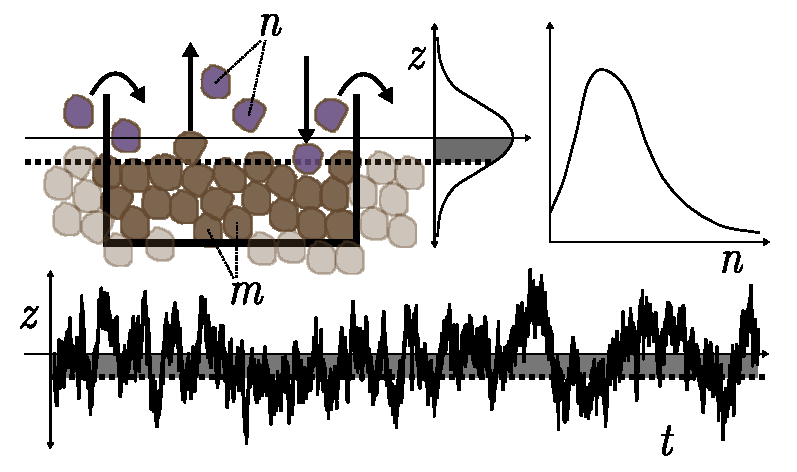
\includegraphics[width=\linewidth,keepaspectratio]{./figures/definition-combo.pdf}
  \vspace{-1.0cm}
  \caption{Definition sketch of a control volume containing $n$ moving grains and $m$ resting grains. Migration, entrainment, and deposition processes are represented by curved arrows, and the bed elevation at some instant is depicted by dotted line. The bed is presented in a degraded state, where $m<m_0$. The distributions of $n$ and $m$ are indicated in the upper right panel, while the bottom panel is a time-series of bed elevations (\ref{eq:ele}).}
  \label{fig:concept}
\vspace{-0.75cm}
\end{figure}

The populations $n$ and $m$ provide the bulk bedload flux $q_s$ and the local bed elevation $z$.
The mean bedload transport rate is given by $q_s \propto u_s \bra n \ket$, where $u_s$ is the characteristic velocity of moving bedload and $\bra n \ket = 
\sum_{n,m}nP(n,m) $ is the mean number of grains in motion \citep[e.g.][]{Charru2004, Ancey2008, Furbish2012a}.
The bed elevation is related to $m$ though the packing geometry of the bed.
To derive this, we prescribe a mean number of grains at rest $m_0$ and introduce a packing fraction $\phi$ of grains in the bed \citep{Torquato2018}.
Considering a two-dimensional bed \citep[e.g.][]{Einstein1950, Paintal1971}, the deviation from the mean bed elevation is
\be z(m) = \frac{\pi a^2}{\phi L}(m-m_0) = z_1(m-m_0). \label{eq:ele}\ee
The constant $z_1 = \pi a^2/(\phi L)$ is an important scale of the problem. 
$z_1$ is the magnitude of bed elevation change (in an average sense across the control volume) associated with the addition or removal of a single grain.
We write the rates of the four possible transitions as \citep[e.g.][]{Ancey2008}:
\begin{align}
 &R_{MI}(n+1,m|n,m) = \nu & \text{migration in}, \label{eq:rate1}\\
 &R_E(n+1,m-1|n,m) =\lambda(m) + \mu(m) n  & \text{entrainment},  \label{eq:rate2}\\
 &R_D(n-1,m+1|n,m) =\sigma(m) n & \text{deposition},\label{eq:rate3}\\
 &R_{MO}(n-1,m|n,m) =\gamma n & \text{migration out\label{eq:rate4}}.
\end{align}
These rates are independent of the past history of the populations and depend only on the current populations $(n,m)$. 
As a result, the system is Markovian \citep[e.g.][]{Cox1965, VanKampen1992}, meaning time intervals between subsequent transitions are exponentially distributed \citep[e.g.][]{Gillespie2007}.

In (\ref{eq:rate1}-\ref{eq:rate4}), $\nu$ and $\gamma$ are constants characterizing migration rates of individual grains into and out of the volume. 
They lack any dependence on the populations $n$ and $m$.
In contrast, $\lambda(m)$, $\mu(m)$, and $\sigma(m)$, characterizing the entrainment, collective entrainment \citep[e.g.][]{Ancey2008, Heyman2013, Heyman2014}, and deposition rates of individual grains are considered to depend on $m$.
As is well-known, bed elevation changes modify the likelihood of entrainment and deposition in a negative feedback \citep{Sawai1987, Wong2007}; that is, aggradation increases the likelihood of entrainment, while degradation increases the likelihood of deposition.
\citet{Wong2007} concluded that bed elevation changes induce an exponential variation in entrainment and deposition probabilities, while \citet{Sawai1987} concluded that the variation is linear.
For simplicity, we incorporate the scaling of \citet{Sawai1987} and note its equivalence to the \citet{Wong2007} scaling when bed elevation changes are small.
Because experimental distributions of bed elevations are usually symmetrical, \citep{Wong2007, Singh2009, Martin2014}, we expect the erosion and deposition feedbacks to be anti-symmetrical.
That is, as bed elevation changes drive up (down) erosion rates, so they drive down (up) deposition rates to the same degree.


% set up the m dependence of the rates
Summarizing these ideas, the entrainment and deposition rates can be written $\chi(m) = \chi_0(1\pm z_1 z(m)/(2l)^2)$, where $\chi = \lambda, \mu, \sigma$, and the entrainment parameters take the plus sign, while deposition takes the minus, and we have introduced a length scale $l$.
As we'll see, the variance of bed elevation turns out to be given by $\text{var}(z) = (l / z_1)^2$. Accordingly, $l$ characterizes the range of bed elevation variations, which could be interpreted as the active layer depth \citep[e.g.][]{Church2017}.
Another perspective is that $l$ is the distance of bed elevation change at which the entrainment and deposition rates are significantly affected.
With these substitutions, the local bed elevation-dependent entrainment and deposition rates (\ref{eq:rate2}-\ref{eq:rate3}) can be written:
\begin{align}
R_E(n+1,m-1|n,m)&=[\lambda_0 + \mu_0 n]\Big[1 + \frac{z_1z(m)}{(2l)^2}\Big], && &\text{entrainment}, \label{eq:rate5}\\
R_D(n-1,m+1|n,m)&=\sigma_0 \Big[1-\frac{z_1z(m)}{(2l)^2}\Big]n, && &\text{deposition}. \label{eq:rate6}
\end{align}
At $z(m)=0$, the rates reduce to those of the \citet{Ancey2008} theory.
Away from this elevation, entrainment and deposition are alternatively suppressed and accentuated depending on the sign of $z(m)$.


In terms of the transition rates (\ref{eq:rate1}-\ref{eq:rate6}), we can obtain the Master equation for the probability flow using the forward Kolmogorov equation $\partial P(n,m;t)/\partial t = 
\sum_{n',m'} R(n,m)P(n',m';t)$ \citep[e.g.][]{Cox1965, Gillespie1992, Ancey2008} as 
\begin{multline}
 \frac{\partial P}{\partial t}(n,m;t) =  
\nu P(n-1,m;t) + 
\{\lambda(m+1) + [n-1]\mu(m+1)\}P(n-1,m+1;t)\\ + 
[n+1]\sigma(m-1)P(n+1,m-1;t) + 
[n+1]\gamma P(n+1,m;t) \\- 
\{ \nu + \lambda(m) + n\mu(m) + n\sigma(m) + n \gamma \}P(n,m;t).
 \label{eq:master}
\end{multline}
The joint probability distribution $P(n,m;t)$ solving this equation will fully characterize the statistics of $n$ and $m$.
We anticipate that solutions will adjust from the initial conditions to a steady-state distribution $P_s(n,m)$, independent of time, if the constant factors in the transition rates are representative of steady bedload transport conditions.
This Master equation describes a two-species stochastic birth-death model \citep[e.g.][]{Cox1965} of a type well-known in the population ecology literature \citep[e.g.][]{Pielou1977, Swift2002}.
In our context, the two species are the moving and stationary grains in the volume.

\section{Numerical simulations}

Unfortunately, (\ref{eq:master}) does not appear to admit an analytical solution (but see \citet{Swift2002} for a standard method which fails in this case).
The difficulty stems from the product terms between $n$ and $m$.
In response, we numerically simulate (\ref{eq:master}) using the Gillespie algorithm \citep{Gillespie1977, Gillespie1992, Gillespie2007}.
The Gillespie algorithm leverages the defining property of a Markov process: when transition rates do not depend on the past, time intervals between transitions are exponentially distributed \citep[e.g.][]{Cox1965}.



\begin{wraptable}{l}{0.5\textwidth}
	\caption{Parameters from \citet{Ancey2008} experiments describing the rates of migration in, entrainment, deposition, and migration out when $z(m)=0$. All units are $s^{-1}$ (probability/time). In our model, bed elevation changes modulate these rates in accord with (\ref{eq:rate1}-\ref{eq:rate6}).}\label{tab:anceyparams}
	\begin{tabular}{cccccc} \\ 
		\toprule  
		Flow & $\nu$ & $\lambda_0$ & $\mu_0$ & $\sigma_0$ & $\gamma$ \\
		\midrule
		(a) & 5.45  & 6.59  & 3.74 & 4.67 & 0.77 \\
		\midrule
		(g) & 7.74  & 8.42  & 4.34 & 4.95 & 0.56 \\
		\midrule
		(i) & 15.56 & 22.07 & 3.56 & 4.52 & 0.68 \\
		\midrule
		(l) & 15.52 & 14.64 & 4.32 & 4.77 & 0.48 \\
		\midrule
		(n) & 15.45 & 24.49 & 3.64 & 4.21 & 0.36 \\
		\bottomrule
	\end{tabular}
\end{wraptable} 

Therefore, to step the Markov process through a single transition, it's enough to draw a random value from the exponential distribution of transition intervals to determine the time of the next transition.
Then, drawing another random value to choose the type of transition which occurs, using the relative probabilities (\ref{eq:rate1}-\ref{eq:rate6}), the transition can be enacted by shifting $t$, $n$ and $m$ by the appropriate values (i.e., entrainment is $m\rightarrow m-1$ and $n \rightarrow n+1$, and so on).
This procedure can be iterated to form an exact realization of the stochastic process \citep[e.g.][]{Gillespie2007}.

In this way, we simulated 5 flow conditions with 10 different values of $l$ taken across a range from $l=a$ (1 grain radius) to $l=10a$ (10 grain radii).
These values lie in the range exhibited in the majority of available experimental data \citep{Wong2007,Singh2009,Martin2014}.
For the migration, entrainment, and deposition parameters at each flow condition $(\nu, \lambda_0, \mu_0, \sigma_0, \gamma)$, we used values measured by \citet{Ancey2008} in a series of flume experiments.
These are summarized in table \ref{tab:anceyparams}.
Flow conditions are labeled (a), (g), and so on, roughly in order of increasing bedload flux (see \citet{Ancey2008} for more details). 
However, our conclusions are not dependent on these parameters.
In all simulations, we take the packing fraction $\phi = 0.6$, a typical value for a pile of spheres \citep[e.g.][]{Bennett1972}, and set $L = 22.5$cm and $a = 0.3$cm, in accord with the \citet{Ancey2008} experiments.
Each simulation was run for $1500$hrs of virtual time, a period selected to ensure convergence of the resting time statistics.

\section{Results}

Our simulations show noisy time-series of bedload activities and bed elevations (as seen in the bottom panel of figure \ref{fig:concept}).
From our chosen initial conditions, all simulations show a rapid attainment of steady state conditions followed by a steady-state stochastic dynamics of $n$ and $m$, supporting a time-independent joint distribution $P_s(n,m)$. 
We compute this joint distribution by counting occurrences of the states $(n,m)$ in the simulated time series.
From this joint distribution we compute marginals $P(n)$ and $P(m)$ as explained in section \ref{sec:theory}.

\begin{wrapfigure}{r}{0.5\textwidth}
	\centering
	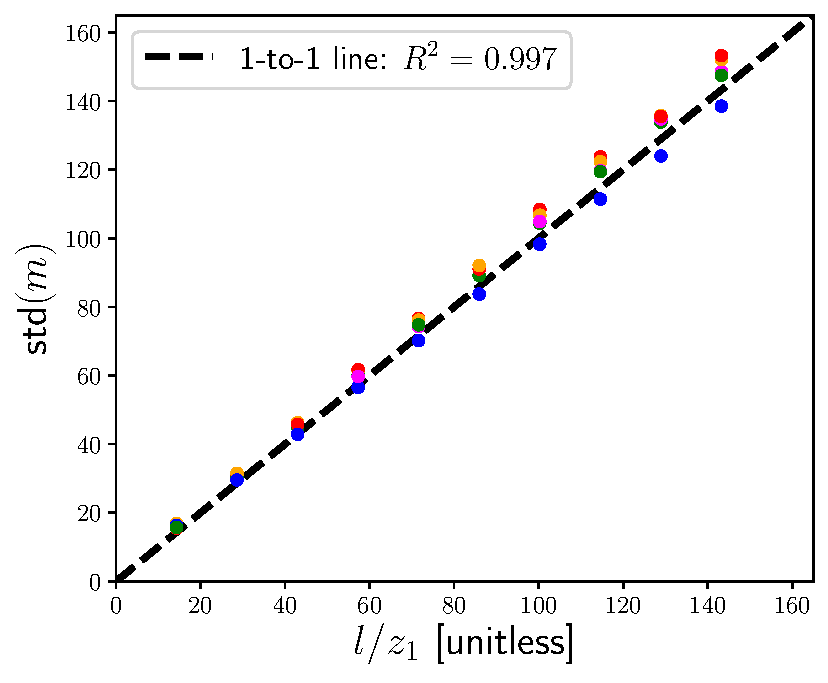
\includegraphics[width=0.5\textwidth,keepaspectratio]{./figures/variance.pdf}
	\caption{Data from all simulations is plotted to show that $l$ controls deviations of bed elevations: $\text{var}(m) = (l/z_1)^2$. }
	\label{fig:var}
\end{wrapfigure}


Some of these marginal distributions are displayed in figure \ref{fig:pdfs}.
Neglecting changes in bed elevation, \citet{Ancey2008} analytically derived negative binomial (NegBin) distributions for the bedload activity $n$, and this functional form seems preserved after including bed elevation changes, because all our computed distributions admit clean NegBin fits (figure \ref{fig:pdfs}a).
For $m$, our computations show Gaussian distributions (figure \ref{fig:pdfs}b), consistent with our assumptions about the scaling of erosion and deposition rates with bed elevation changes \citep[e.g.][]{Wong2007}.

\begin{figure}[t!]
	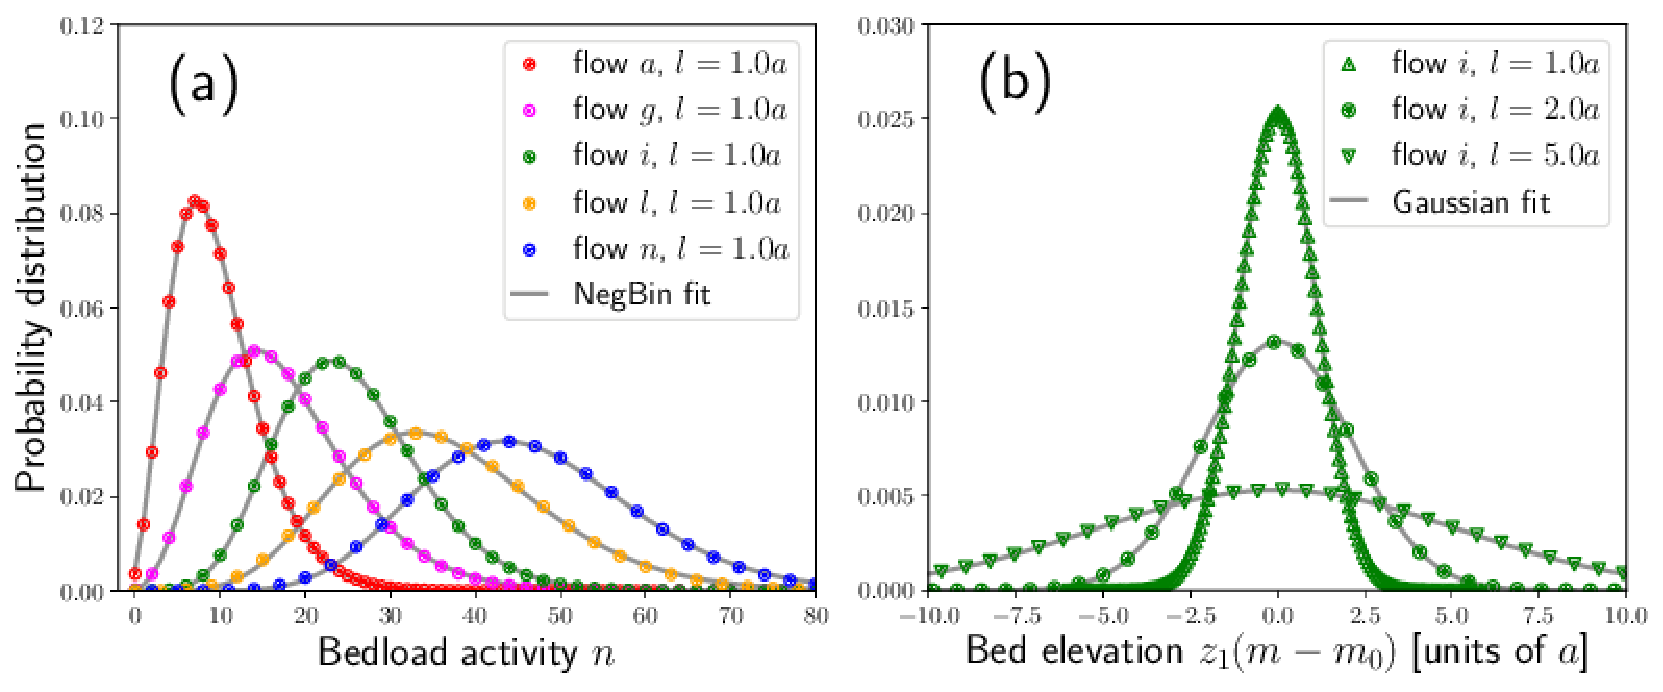
\includegraphics[width=\linewidth,keepaspectratio]{./figures/montage2.pdf}
	\caption{Marginal distributions of $n$ and $m$ for a subset of simulations. Some points have been omitted for clarity.}
	\label{fig:pdfs}
\end{figure}

From the marginal distributions, we calculate means and variances of bedload activity ($n$) and elevation ($m$).
The mean bed elevation is $m_0$, the parameter in (\ref{eq:ele}). $m$ fluctuates around this value because it sets the equilibrium position of the elevation-related feedbacks within (\ref{eq:ele}).
The variance of $m$ appears given by $z_1^2 \text{var}(m) = l^2$, as indicated in figure \ref{fig:var}, consistent with our interpretation of $l$ as a measure of bed elevation fluctuations.
The moments of $n$ are more difficult to understand.
Without dwelling on the issue, the moments of $n$ shift with the ratio $l/z_1$ as a result of the feedback between bed elevation changes and bedload transport.

Now we describe the analysis of bedload resting times from time-series of $m$.
Following \citet{Voepel2013} and \citet{Martin2014}, we concentrate on a particular bed elevation $m'$, and find all time intervals separating deposition events at $m=m'$ from erosion events at $m=m'+1$.
These are the return times from above of the bed conditional to the elevation $m'$.
Binning these conditional return times (with logarithmic bins) and counting the occurrences in each bin, we obtain a non-exceedance distribution of return times $t_r$ held conditional to the elevation $m'$: $P(T>t_r|m')$.
Using the marginal probability distribution of bed elevations, we derive the unconditional non-exceedance distribution of resting times as a sum over all elevations \citep{Yang1971, Nakagawa1980, Voepel2013, Martin2014}:
\be P(T>t_r) = \sum_{m'} P(m') P(T>t_r|m') .\ee
Some of these results are displayed in figure \ref{fig:cdfs}.
In contrast to earlier works our analysis does not require binning over the elevation, since our elevation series is discrete (multiples of $z_1$).
Comparing panels (a) and (c) shows the resting time distributions scale with the intensity of bedload transport and the standard deviation of bed elevations ($l$) differently.
However, as shown in panels (b) and (d), a characteristic timescale $T_0$ can be found to collapse away both of these differences.
\begin{figure}[t!]
	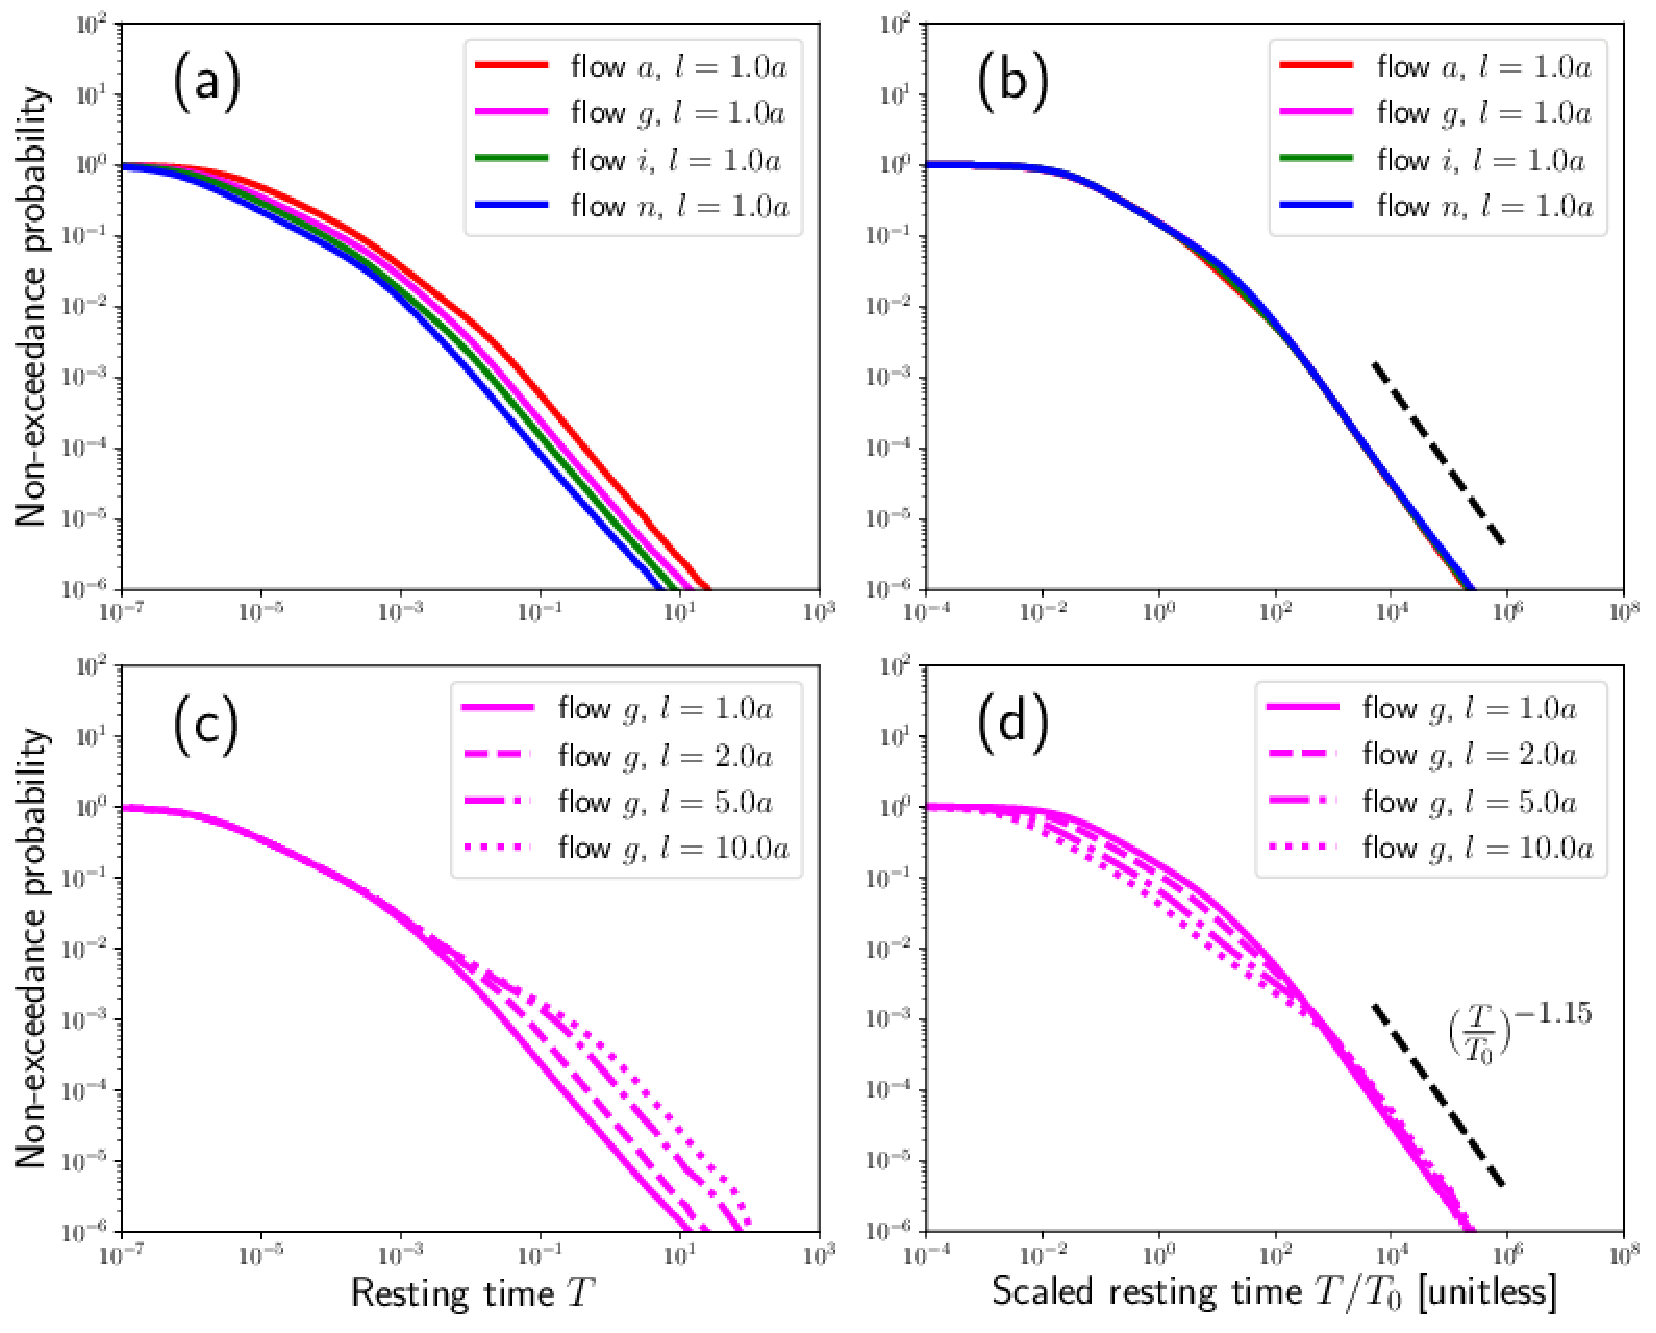
\includegraphics[width=\linewidth,keepaspectratio]{./figures/montage1.pdf}
	\caption{Resting time statistics scale differently with transport conditions and the bed elevation variance. Panel (a) shows differing flow conditions at a fixed $l$ value, while panel (c) shows fixed flow conditions at differing $l$. When scaled by $T_0$ (\ref{eq:time}), both types of difference collapse in the tails of the distributions, as shown in panels (b) and (d). In panels (b) and (d), the black dotted lines indicate a power law decay of the collapsed tails having parameter $\alpha\approx1.18$ .}
	\label{fig:cdfs}
\end{figure}

We can obtain $T_0$ heuristically by finding a characteristic speed of bed elevation change.
Formally, the mean erosion rate is $E = \sum_{n,m}R_E(n,m)P(n,m)$.
This is the number of grains leaving the bed per unit time.
Since the removal of a single grain changes the bed elevation by $z_1$, bed elevations change with a characteristic speed $z_1 E$.
Since the characteristic deviation of elevation is $l$, the time required for the bed to shift through a characteristic deviation is
\be T_0 = \frac{l}{z_1 E}.\label{eq:time}\ee
When scaling the resting time by this $T_0$, we obtain the collapse shown in figure \ref{fig:cdfs}.
Using the log-likelihood estimation described by \citet{Newman2005}, we estimate for all return times satisfying $T/T_0 > 10^3$, the resting time non-exceedance distributions decay as a heavy-tailed power law with parameter $\alpha = 1.18 \pm 0.32$.
%\alpha = 1.182 \pm 0.318

\section{Discussion}

% A) discuss the historical context and the classic related work

\citet{Einstein1937} created the first theory of individual bedload motions and diffusion, and his ideas can be viewed as the historical nexus of an entire paradigm of research which extends into the present day \citep[e.g.][]{Hubbell1964,Yano1969, Nakagawa1976,Hassan1991,Ancey2008,Phillips2013,Martin2014, Furbish2012, Heyman2016, Bradley2017}.
Works in this paradigm attempt to understand properties of bedload transport such as bulk fluxes or diffusion by applying stochastic concepts to individual motions.
With a few exceptions \citep[e.g.][]{Yang1971,Nakagawa1980,Wu2019}, existing theories are spatially one-dimensional, concentrating on the motion of grains in the downstream direction but neglecting the vertical dimension, wherein bed elevation changes can imply sediment burial \citep[e.g.][]{Voepel2013,Martin2014} and modify the mobility of surface grains \citep[e.g.][]{Yang1971,Nakagawa1980,Sawai1987,Wong2007}.

% B) Discuss how your work links to the historical context
In this work, we have built upon this body of research to create a theory describing bedload transport and bed elevation changes from a stochastic concept of individual bedload motions.
In particular, we have generalized the \citet{Ancey2008} bedload theory to include bed elevation changes, incorporating feedbacks between the local bed elevation and the instantaneous erosion and deposition rates \citep[e.g.][]{Wong2007} to form a joint description of bulk bedload fluxes and bed elevation changes.
Our simulations reveal negative binomial distributions for bedload activities and normal distributions for bed elevations, reproducing a wide set of experimental findings \citep{Ancey2008, Heyman2016, Wong2007, Singh2009, Martin2014}.
Two key contributions of this work are: (1) it predicts resting time distributions for sediment undergoing burial, which are otherwise important to bedload diffusion, difficult to measure, and poorly understood \citep[e.g.][]{Voepel2013, Martin2014, Bradley2017}; and (2) it provides a basis for further developments in the Einstein paradigm which include a vertical dimension of bed elevation dynamics.
In this section, we will link our work to earlier research and detail these two contributions. 

% C) discuss the link to Martin and to Ancey
Our theory reproduces earlier descriptions of bedload activities by \citet{Ancey2008} and bed elevations by \citet{Martin2014} after taking mean field limits of (\ref{eq:master}).
The \citet{Ancey2008} bedload theory is obtained when bed elevation fluctuations $\delta m$ are small: $m \approx m_0$.
Taking account of this change in (\ref{eq:master}) derives the master equation of \citet{Ancey2008} for the bedload activity distribution $P(n,t)$.
Similarly, the \citet{Martin2014} bed elevation theory is obtained when bedload activity fluctuations $\delta n$ are small: $n \approx \bra n \ket$.
In this case, identifying the mean entrainment and deposition rates as $E =\lambda_0 + \mu_0 \bra n \ket$ and $D = \sigma_0 \bra n \ket$, and using the steady-state transport condition $E=D$ \citep[e.g.][]{Einstein1950} obtains
\be \frac{\partial}{\partial t}P(m,t) =  E \Big\{ \Big[1 +\Big(\frac{z_1}{2 l}\Big)^2m\Big]P(m+1,t) +  \Big[1 -\Big(\frac{z_1}{2 l}\Big)^2m\Big]P(m-1,t) - 2P(m,t)\Big\}, \label{eq:ou}\ee
This is a discrete state analogue of the mean-reverting random walk used by \citet{Martin2014} to model bed elevation changes.

% D) Discuss differences with the martin theory
Differences between our bed elevation statistics and those predicted by \citet{Martin2014} (i.e., equation \ref{eq:ou}) are induced by $\delta n$ -- the bedload activity fluctuations.
When bedload fluctuations are relatively small $|\delta n/\bra n \ket|<1,$ we expect the \citet{Martin2014} theory to be an excellent description of bed elevation time series, as it follows naturally from a mean field limit of our theory based upon individual sediment motions.
However, bedload fluctuations are often relatively large.
For example, in the \citet{Ancey2008} experiments, $|\delta n/\bra n \ket|$ takes instantaneous values of up to $3$ or $5$.
When this is true we expect the approximation (\ref{eq:ou}) provides a poor description of bed elevation statistics.
Although (\ref{eq:ou}) and (\ref{eq:master}) both generate Gaussian bed elevation distributions, they imply very different correlations in the bed elevation time series.
The Ornstein-Uhlenbeck process used by \citet{Martin2014} (\ref{eq:ou}) has an exponential correlation function \citep[e.g.][]{Horsthemke1984,Risken1989}.
In contrast, we find correlation functions from our simulations which decay more slowly than exponential.
This implies bedload fluctuations can induce longer correlations in bed elevation time-series than an Ornstein-Uhlenbeck theory can produce.

% E) discuss your key conclusions on resting time distributions and bedload diffusion / discuss relationship to field studies and laboratory experiments
Our computed resting time distributions (figure \ref{fig:cdfs}) show asymptotic power law tails with parameter $\alpha = 1.18 \pm 0.32$ after scaling by $T_0$.
%These decay more rapidly than those with $\alpha \approx 1$ identified by \citet{Martin2014}.
For a general power law, if $\alpha>1$, neither the mean or variance of the resting time will converge, while if $1<\alpha <2$, the mean will converge while the variance will not \citep[e.g.][]{Bradley2017}.
Within our computational uncertainty, which stems from the finite duration of our simulations and the log-likelihood estimation \citep[e.g.][]{Newman2005}, we are unable to conclude whether the mean resting time will diverge, but we can conclude the variance will diverge.
This is a violation of the central limit theorem for the bedload motion, and we can expect anomalous super-diffusion at long timescales.
According to \citet{Weeks1998}, if the step length distribution has a light tail \citep[e.g.][]{Hassan2013}, our computed power-law resting times are sufficiently heavy-tailed to imply diffusion scaling as either $\sigma_x^2 \propto t^{3-\alpha} \approx t^{\{1.82 \pm 0.32 \}}$ or $\sigma_x^2 \propto t^{2\alpha} \approx t^{\{3.64\pm 1.28\}}$ at asymptotically large times \citep[e.g.][]{Bradley2017}.
In either case, the process of sediment burial induces an extreme super-diffusion of bedload: at long timescales, some grains will continue to transport downstream in alternate motion-rest sequences while others will become trapped under the bed for relatively very long periods of time, driving a rapid spreading of the population.














\begin{comment}











However, we emphasize this is long-time diffusive scaling only.
In fact, the conclusions of \citet{Weeks1998} are derived entirely from asymptotic arguments.
\citet{Nikora2001,Nikora2002} set an expectation of at least three ranges of bedload diffusion called local, intermediate, and global as a result of the scale dependence of the various processes at play in bedload motions, such as collisions, turbulent fluctuations, and burial.
These three ranges have been captured by several theoretical models \citep[e.g.]{Bialik2012,Zhang2012,Fan2016}.
While the transition point from local to intermediate scales is relatively well-understood, and there is some theoretical support for the notion of super-diffusion in the local range and normal diffusion in the intermediate range, the transition point between the intermediate and global ranges has so far, to our knowledge, defied theoretical description.
Given the mounting theoretical arguments here and elsewhere \citep[e.g.][]{Martin2014,} and experimental support for global range super-diffusion \citep[e.g.][]{Phillips2013,Bradley2017,Pretzlav2016,Olinde2015,Voepel2013}, and the relative lack of understanding of the transition point between the intermediate and global ranges, we believe understanding of diffusion for many timescal




We predict heavy-tailed power law resting times with parameter $\alpha \approx 1.18$ as a result of sediment burial.
The tails of these distributions show near-perfect collapse upon scaling resting times by the factor $T_0 = l/(z_1 E)$, a characteristic timescale of bed elevation change, and we find the asymptotic behaviors occur for $T/T_0>10^3$.
We note 


In contrast, \citet{Martin2014} 



In addition, since $1 \leq \alpha \leq 2$, tracer positions will have a convergent mean \citep[e.g.][]{Weeks1998, Bradley2017}.
For comparison, \citet{Martin2012} found $\alpha = 0.85$ from a three-dimensional flume experiment,  \citet{Voepel2013} found $\alpha = 0.88$ in data from the field study of \citet{Habersack2001},
\citet{Phillips2013} found $\alpha = 1.12$ from their field study, \citet{Martin2014} found $\alpha \approx 1.0$ from their simulations and two-dimensional flume experiments, and \citet{Bradley2017} found $\alpha = 0.67$ from field data. 
All of these values imply anomalous diffusion, like our simulation results, while only \citet{Phillips2013} and perhaps \citet{Martin2014} predict convergent means consistent with our results.
These discrepancies may stem from our assumption that burial is the source of heavy tails in these field data. 
We have analyzed return periods of the bed elevation, but as noted by \citet{Bradley2017}, 
other return periods impede tracer motions in gravel bed rivers, such as the deposition of sediment on top of floodplains \citep[e.g.][]{Bradley2013}, or on top of high bars in the bends of a stream \citep[e.g.][]{Bradley2017}.

























Given this conclusion, we find it shocking that our resting time distributions (figure \ref{fig:cdfs}) show obvious accord with those of \citet{Martin2014}.
Seemingly, the correlation structure of the bed elevation time series does not modify the resting time distributions for sediment undergoing burial.
Resting time distributions appear to be universal (in scaled time $T/T_0$) across bedload transport conditions, and indeed across coupling bed elevation statistics to bedload transport.

The universal resting time distributions obtained from our theory which correspond to those of \citet{Martin2014} 
In fact, there are many examples in the physics literature where extremal properties of a random walk (first passage times, return times, maxima) show universal characteristics independent of underlying statistics.
We hypothesize this is the case in  

%Given this conclusion, we find it shocking that our resting time distributions (figure \ref{fig:cdfs}) show obvious accord with those of \citet{Martin2014}, apart from the imperfect collapse \citet{Martin2014} display in the tails of their scaled distributions.
%The imperfect collapse may be explained by their scaling by a bed activity scale $1/a$ (equivalent to $1/(2E)$ in our notation), instead of a scale involving the bed activity and the variance of bed elevations (such as our $T_0$), since this latter quantity slightly varied across their experiments.
%The correspondence of their resting time distributions with ours despite their simplification of the correlation structure of the bed elevation time-series, which is actually non-exponential and linked to bedload fluctuations, is more remarkable and difficult to understand.

Now we discuss the universality of our resting time results which ties into their correspondence with \citet{Martin2014}, and we analyze implications for bedload diffusion.






, which emerges despite differences in bedload fluctuation induced correlations in bed elevation time series,



are a consequence of the so-called Sparre-Andersen theorem pertaining to extreme events of a random walk.
The Sparre-Andersen  \citep{Feller1968, Redner2007}.




Given this conclusion it appears shocking that our resting time distributions show a universal character which is independent of the magnitude of bedload fluctuations and the relatively long correlations they induce in the bed elevation time-series (figure \ref{fig:cdfs}(b)).
In fact, our universal distributions are consistent with those of \citet{Martin2014} as well.

 
Although temporal correlations of the bed elevation time-series appear directly affected by bedload fluctuations, the return time distributions (i.e., the resting times for sediment undergoing burial) are not affected by these fluctuations, so they appear quite similar to the resting times presented by \citet{Martin2014}.



We believe this universality of the return time distributions across bed elevation correlations, and accord between our results and those of \citet{Martin2014} despite their neglect of these correlations, may be a consequence of the Sparre-Andersen theorem pertaining to extreme events of a random walk 









%As a final comment on the relation of our theory to earlier work, we nearly obtain the %bed elevation theory of \citet{Voepel2013} from (\ref{eq:mft}) when the bed elevation %variance becomes very large relative to the elevation change associated with a single %grain, $l\gg z_1$.
%However, to complete the link to \citet{Voepel2013} we need to further prescribe %reflecting boundary conditions \citep[e.g.][]{Weiss1994}, leaving it somewhat %disconnected from our approach.




























% F) discuss scope for extension of the model

Finally, we discuss the scope for extension of our model.
The limiting relationship we have shown to \citet{Ancey2008}, and knowledge of several follow-up works to \citet{Ancey2008} \citep[e.g.][]{Ancey2014a, Heyman2014, Heyman2015}, suggest an interesting and potentially useful generalization of our model.
These follow-up works are based on chaining many \citet{Ancey2008} single-cell models together along a line, with migration out of one cell being migration into another, and they provide a framework to study spatial correlations in bedload transport \citep[e.g.][]{Heyman2014,Heyman2015}.
One can imagine using our model (\ref{eq:master}) in the same way, chaining an array of volumes together along a line, generating a stochastic 1D morphodynamics theory ultimately rooted in the foundational ideas of \citet{Einstein1950}, and providing spatial correlations in bed elevation changes and bedload transport.
An obvious issue with this idea is how to parameterize the entrainment and deposition rates within the model in terms of local and non-local bed elevations.
Of course, this has been a longstanding issue in deterministic 1D morphodynamics as well \citep[e.g.][]{Tucker2010}.
We speculate that the stochastic analogue of this issue could be easier to understand.























\end{comment}





\section{Conclusion}


We predict heavy-tailed power law resting times with parameter $\alpha \approx 1.18$ as a result of sediment burial.
The tails of these distributions show near-perfect collapse upon scaling resting times by the factor $T_0 = l/(z_1 E)$, a characteristic timescale of bed elevation change, and we find the asymptotic behaviors occur for $T/T_0>10^3$.


Many open questions remain around the problem of anomalous bedload diffusion.
In this paper, we have made incremental steps forward, by framing sediment burial directly in terms of the sediment transport process.
When burial is a dominant process affecting the motions of individual grains, our results should serve as a prototype of this process, as they're derived under the assumptions of uniform grain size and equilibrium sediment transport in the spirit of \citet{Einstein1950}.
We predict anomalous bedload diffusion $\sigma_x^2 \propto t^{1.85}$ and a convergent mean, corroborating a subset of earlier studies.
Most directly, we have derived the \citet{Martin2014} model as an approximate limit of our more general theory, while we found no connection to the \citet{Voepel2013} model.
In closing, we highlight that other return processes in nature could impart heavy tails to fluvial bed material resting times \citep[e.g.][]{Bradley2017}.
To truly understand anomalous diffusion, we need to pin down these processes, quantify their relative importance, and learn to mix their effects.



\acknowledgments
The simulation code is available upon request from the first author. We would like to thank Shawn Chartrand and Conor McDowell for helpful discussions. 

\bibliography{biblio}

\end{document}




